\documentclass[sigplan]{acmart}

\settopmatter{printacmref=false} % Removes citation information below abstract
\renewcommand\footnotetextcopyrightpermission[1]{} % removes footnote with conference information in first column
\pagestyle{plain} % removes running headers

\usepackage[english]{babel}
\usepackage{listings}
\usepackage{url}

\begin{document}

\title{Implementation of Cholesky Factorization using Intel AVX2s insructions}

\author{Oleksandr Zaytsev}
\affiliation{%
  \institution{Ukrainian Catholic University\\
  Faculty of Applied Sciences}
  \city{Lviv}
  \state{Ukraine}
}
\email{oleks@ucu.edu.ua}

\begin{abstract}
Intel Advanced Vector Extensions (Intel AVX) is a set of instructions for doing Single Instruction Multiple Data (SIMD) operations on Intel architecture CPU\cite{lomont-11}.

In this work I demonstrate how AVX instructions can be used to speed up the execution of widely used numerical algorithms. Cholesky factorization was chosen as an example due to it importance.
\end{abstract}

\keywords{SIMD, AVX, parallel algorithms, numerical methods, Cholesky factorization}

\maketitle

\section{Introduction}
Software packages like R call native functions from LAPACK etc.

\subsection{Cholesky Factorization}
Every symmetric positive-definite matrix $A$ can be decomposed into the product

\[ A = LL^\top \]

Where $L$ is a lower-triandular matrix.

\section{Data generation}
I used R to generate 6 symmetric positive-definite matrices with real-value entries. The matrices are square and have the following $250, 500, 1000, 2500, 5000, 7500$ rows respectively. These matrices are then stored in binary files and loaded by other modules of this project.

I chose the approach of pre-generated matrices as opposed to the idea of generating a new matrix for each experiment, because this way the measurements will be more accurate. I compare the performance of two algorithms on exactly the same input.

\section{Implementation}
There are two places in the algorithm that can be parallelized:

\begin{itemize}
\item Inner product
\item Division by diagonal elements
\end{itemize}


\subsection{Dot product}

\lstset {language=C++}
\begin{lstlisting}
double sum;
__m256d ax = _mm256_loadu_pd(&a[0]);
__m256d bx = _mm256_loadu_pd(&b[0]);
__m256d cx = _mm256_mul_pd(ax, bx);
__m256d hsum = _mm256_add_pd(cx,
    _mm256_permute2f128_pd(cx, cx, 0x1));
_mm_store_sd(&sum,
    _mm_hadd_pd(
        _mm256_castpd256_pd128(hsum),
        _mm256_castpd256_pd128(hsum)));
\end{lstlisting}

We start by loading 256-bits (composed of 4 packed double-precision (64-bit) floating-point elements) from array \texttt{a} into ... We do the same for the 4 values from \texttt{b}. Then we perform elementwise multiplication of the two vectors and sum the values of the resulting vector into a scalar.

Intrinsic \texttt{\_mm256\_castpd256\_pd128} is only used for compilation and does not generate any instructions, thus it has zero latency. \texttt{\_mm\_store\_sd} is an SSE2 instruction that stores the lower double-precision floating-point element into memory.

\section{Experimental results}

\begin{figure}[H]
  \begin{center}
  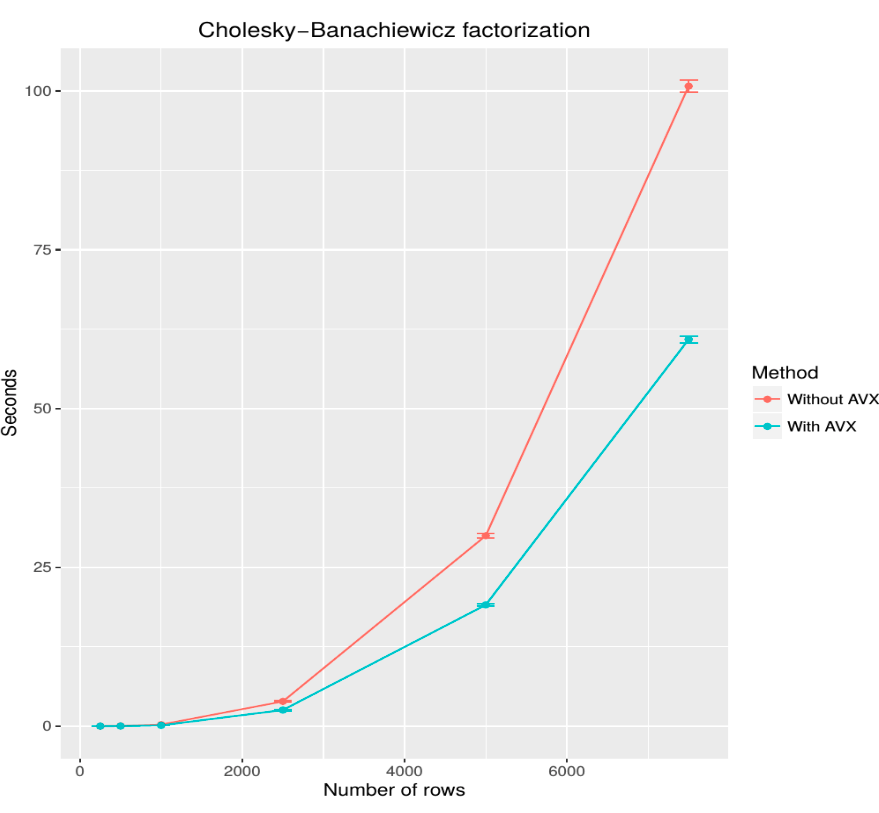
\includegraphics[width=\linewidth]{img/experiment}
  \caption{Comparing the performance of two algorithms}
  \end{center}
\end{figure}


\bibliographystyle{alpha}
\bibliography{CholeskyAVX}

\end{document}